This chapter describes how the use of the different datasets was implemented and presented. The program is divided into two: The backend and the frontend. The structure and functions are provided by the backend, which governs collection and manipulation of data, and the frontend presents the data in a graphical user interface (GUI) using graphs and maps. 
Figure \ref{fig:Conceptual_o} show the conceptual oversights of what this program hopes to achieve. First, the sources are collected and converted into a more convenient format to work with, that format is stored in a database that provides easy access and quick relevant searches. Which is practical for the analytical module which examines the data with various techniques, lastly the results are presented visually.

\begin{figure}[h]
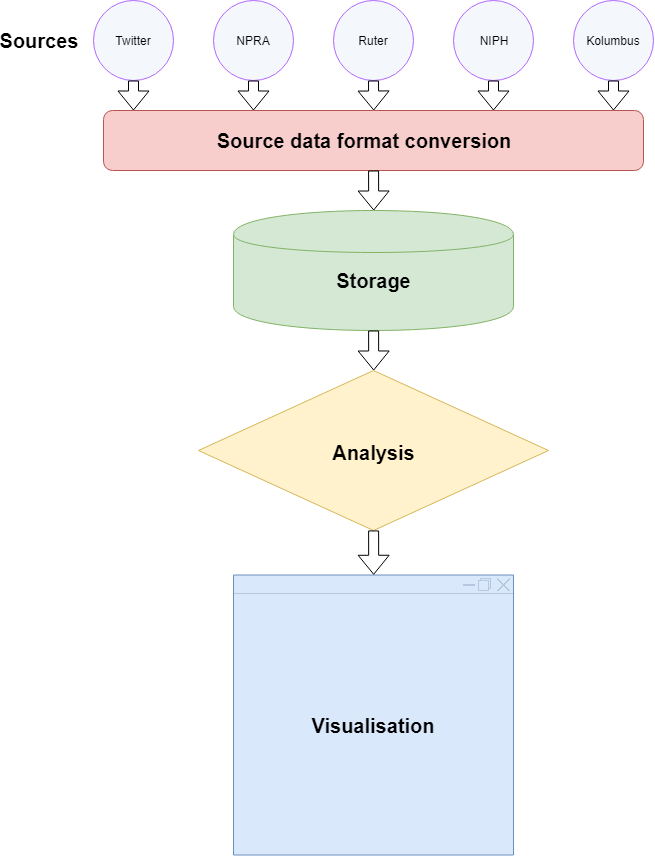
\includegraphics[width=8.5cm]{conseptual_overall}
\centering
\caption{Conceptual oversight}
\label{fig:Conceptual_o}
\end{figure}


\newpage


Figure \ref{fig:program} show the structural relations of the backend and the frontend in a simplified manner. The main module to be run is found in frontend/gui.py, and the system works best with two API keys installed as explained in this chapter. Both the frontend and the backend have more detailed diagrams in their own sub chapters.

\begin{figure}[h]
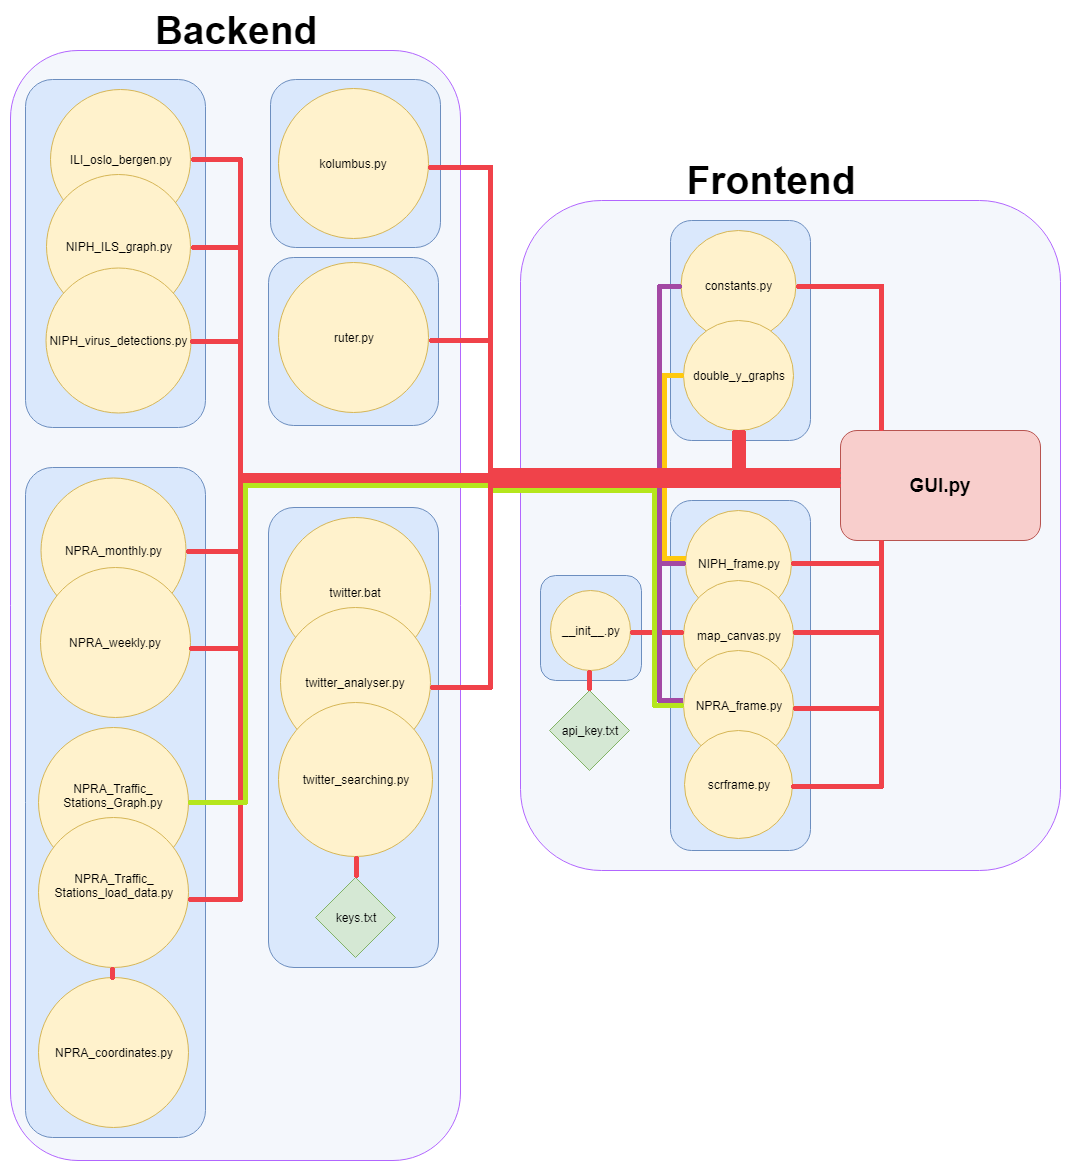
\includegraphics[width=15cm]{program_diagram}
\centering
\caption{Simplification of the overall program structure and relation}
\label{fig:program}
\end{figure}


\newpage



\section{The Backend}
The backend is responsible for providing the frontend all the data and deeper functions it needs to visualize and administrate data to be show in graphs. The backend is partitioned into modules (Python programs/.py files) in their respective directory folder based on each dataset available. Each module may also be run individually for testing and easy viewing purposes. 
The Twitter module is unique as it requires 4 application programming interface (API) keys to work properly. The instructions for this set-up is found in the file README.md in the twitter module's directory. Figure \ref{fig:backend_diagram} shows a diagram of the backend.

\begin{figure}[!htb]
\includegraphics[width=15cm]{backend_diagram}
\centering
\caption{A semi detailed diagram of the Backend structure and functions}
\label{fig:backend_diagram}
\end{figure}

\newpage


\subsection{The Norwegian Institute of Public Health}
There are three different sets of data, which is divided into the separate modules of NIPH\_ILS\_graph.py, NIPH\_virus\_detections.py and ILI\_oslo\_bergen.py located in the same directory backend/NIPH, and they show influenza-like illnesses (ILI), hospitalized viral observations and more detailed ILI from the cities of Oslo and Bergen. The ILS module extract data from a local file, the virus module has it's data hard-coded and the ILI module extracts it's data from a hidden file (more on this in chapter 6), and they all draw their graph(s) using Python's matplotlib library. The graphs can be seen by running the modules individually or in the frontend main program frontend/gui.py's appropriate viewport accessible from the NIPH button. Figure \ref{fig:infstat} show the three last seasons of influenza in regards to observed viral infections. The plotting was done manually as NIPH only provides viral observational data in reports that are in pdf files on their official website\cite{fhi}.

\begin{figure}[h]
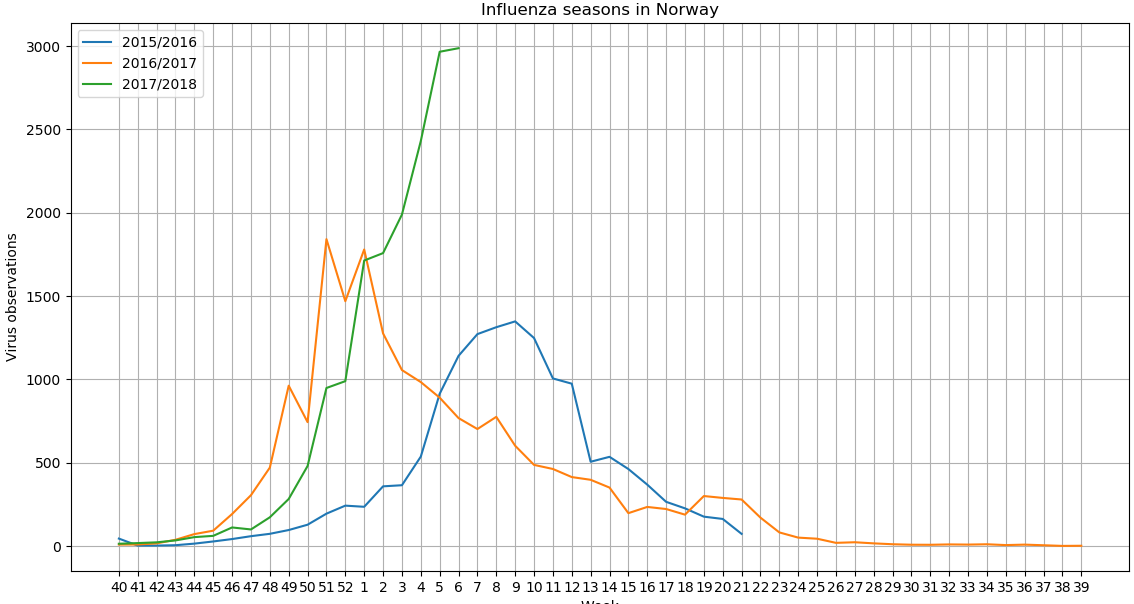
\includegraphics[width=12cm]{influenza_15_till_18}
\centering
\caption{Influenza virus observation}
\label{fig:infstat}
\end{figure}

Figure \ref{fig:ilsstat} shows the influenza-like illnesses (ILI) of the year 2016/2017. This was not done manually as data was provided in a simple .xlsx file which was read using Python's openpyxl module, processed and then drawn as a graph. Figure \ref{fig:ili_oslo} and figure \ref{fig:ili_bergen} show reported ILI from Oslo and Bergen.

\begin{figure}[ht]
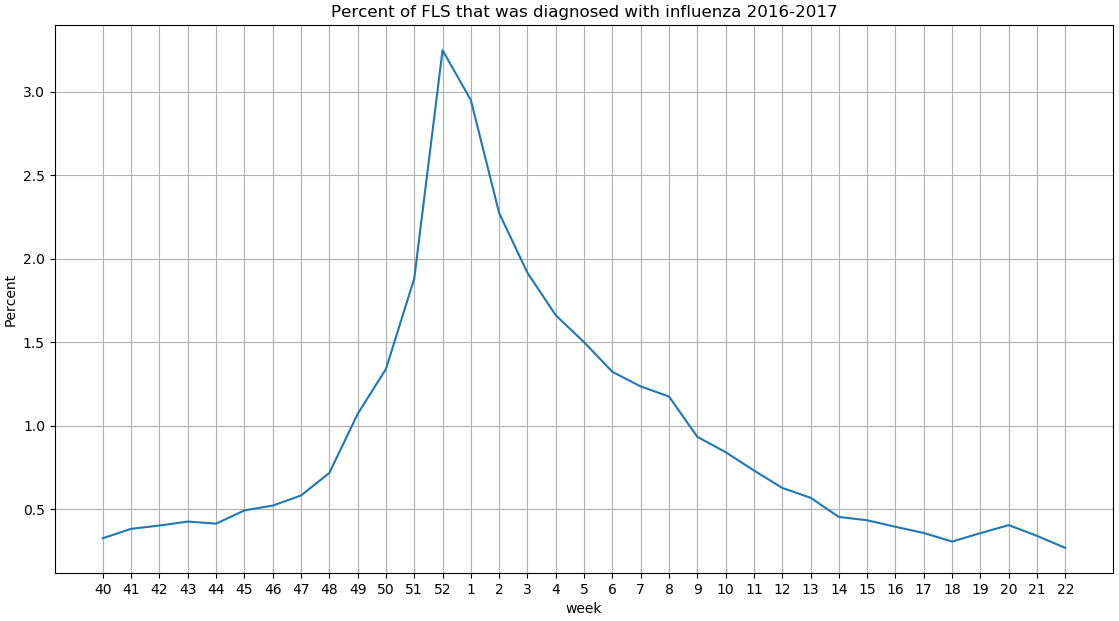
\includegraphics[width=12cm]{ILS_16_till_17}
\centering
\caption{Influenza-like illnesses season 2016/2017}
\label{fig:ilsstat}
\end{figure}

\begin{figure}[ht]
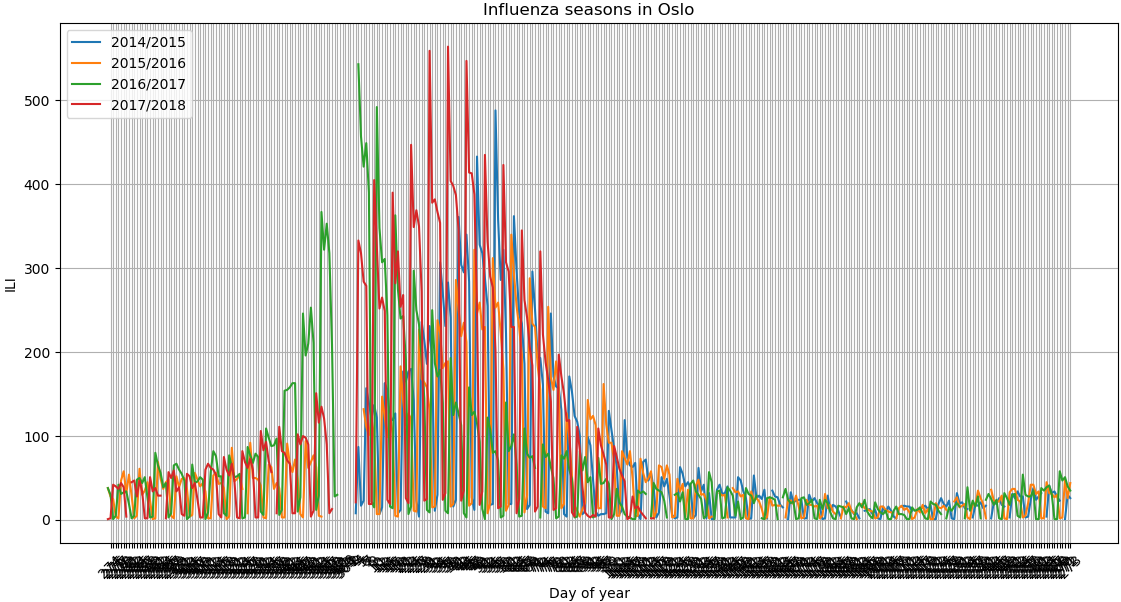
\includegraphics[width=12cm]{ili_daily_oslo}
\centering
\caption{Influenza-like illnesses season 2014-2018 in Oslo}
\label{fig:ili_oslo}
\end{figure}

\begin{figure}[!htb]
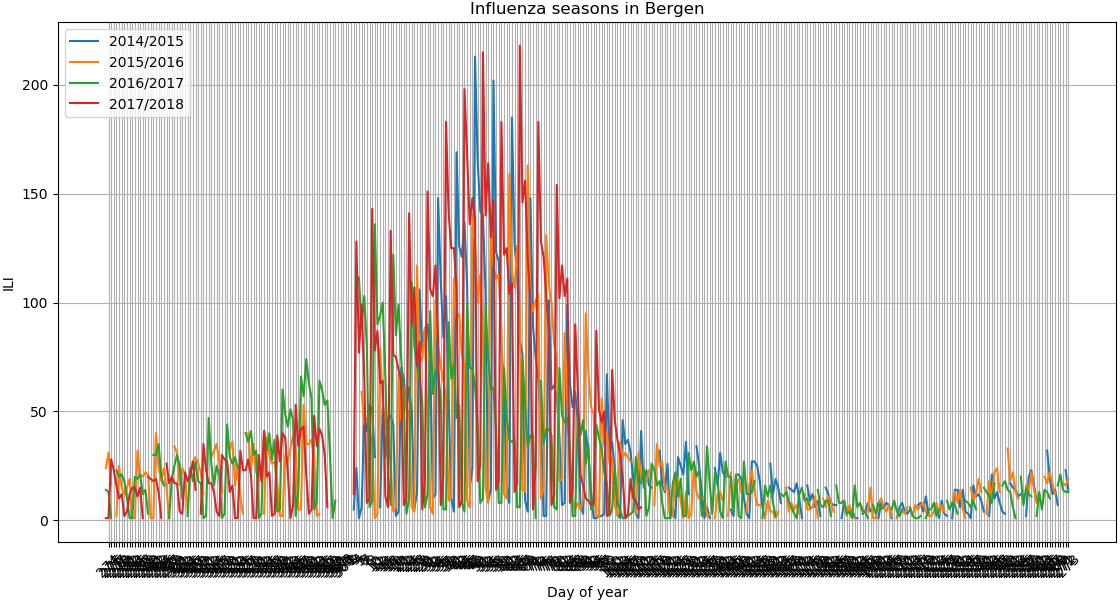
\includegraphics[width=12cm]{ili_daily_bergen}
\centering
\caption{Influenza-like illnesses season 2014-2018 in Bergen}
\label{fig:ili_bergen}
\end{figure}

\newpage









\subsection{The Norwegian Public Roads Administration}
From the .xlsx files provided by the NPRA, simple graphs were created in python showing the total annual traffic on Norwegian roads from 2002 to 2015 on a monthly basis as seen in figure \ref{fig:anualtotal}.

\begin{figure}[ht]
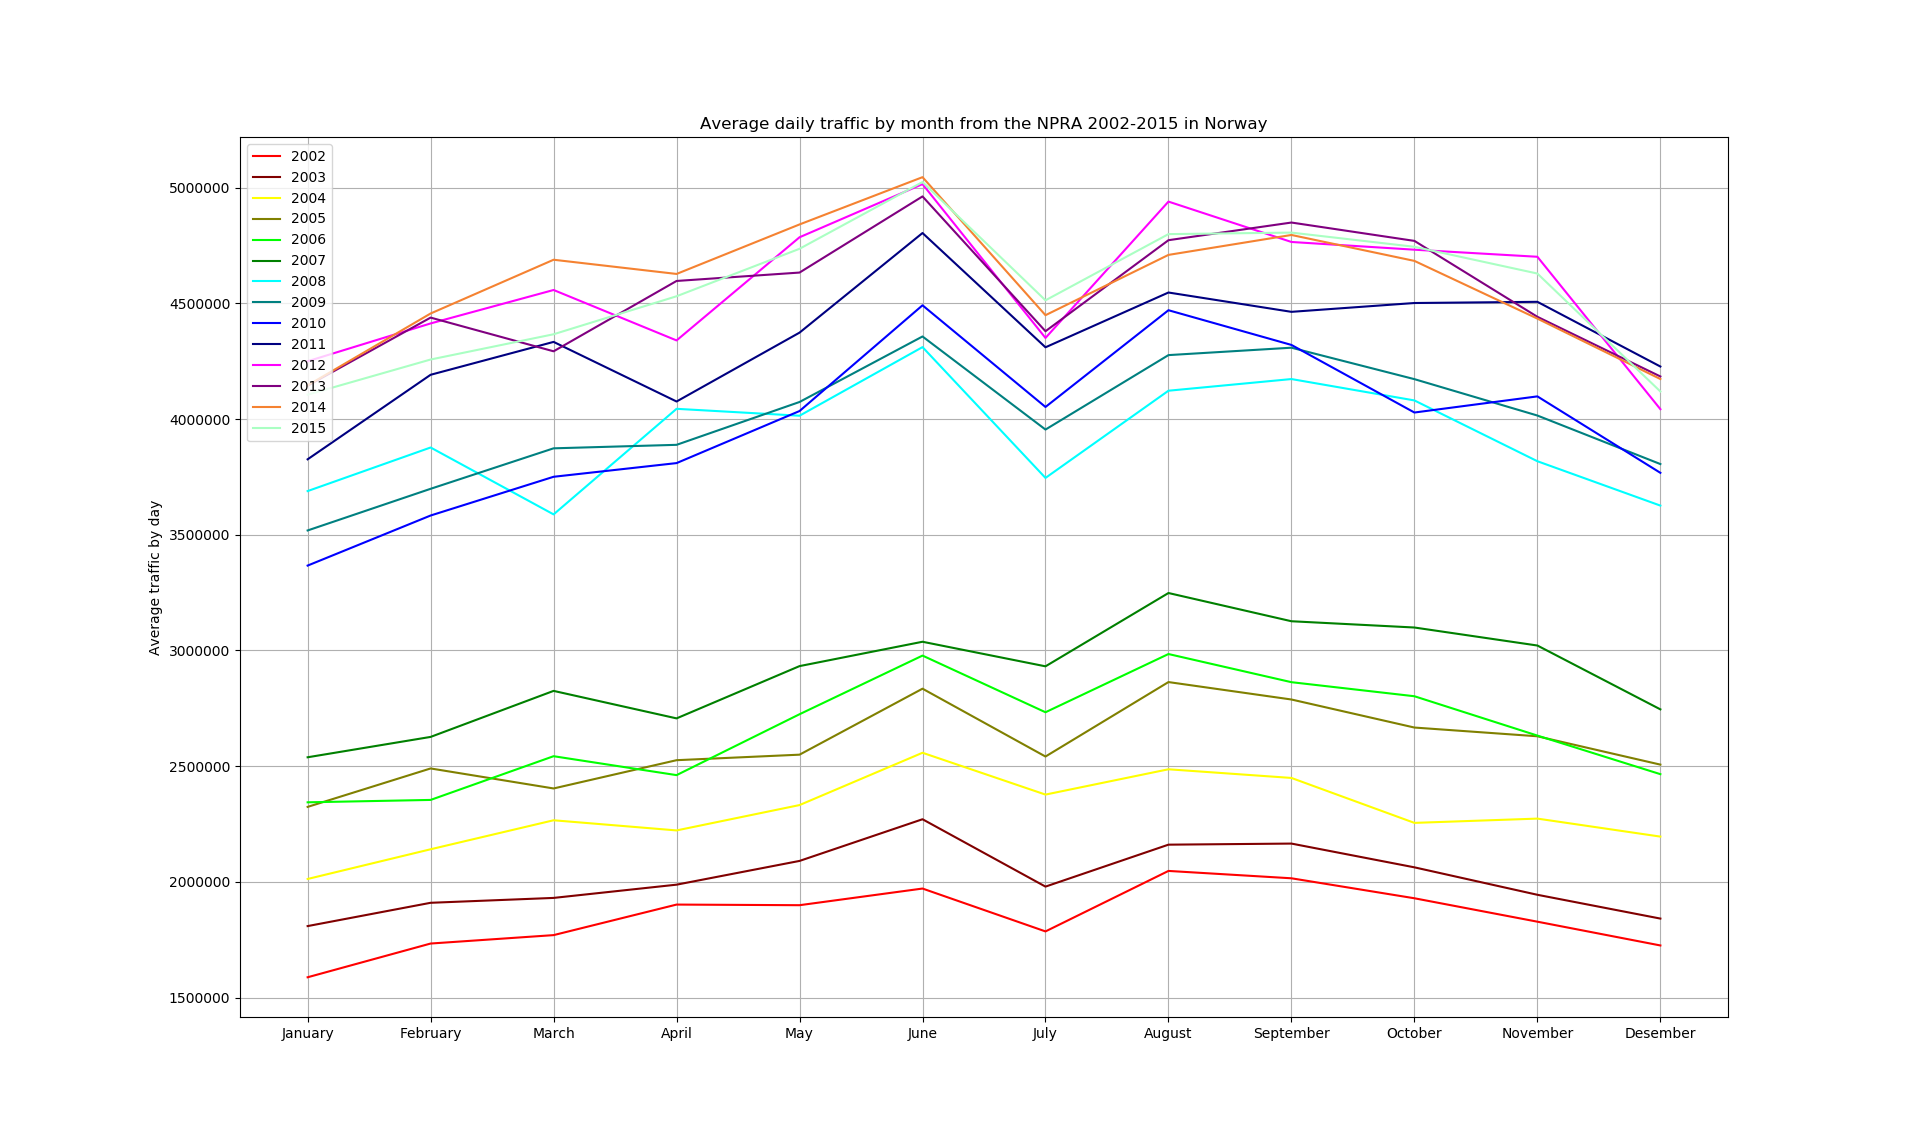
\includegraphics[width=10cm]{xml_02_15_annual_total}
\centering
\caption{Annual traffic 2002-2015}
\label{fig:anualtotal}
\end{figure}

Also derived from this dataset is the annual traffic of the two cities of Bergen and Oslo, which are cities of interest.
%Figure \ref{fig:anualbergen} shows the traffic in Bergen, and figure \ref{fig:anualoslo} show the traffic in Oslo.

%\begin{figure}[ht]
%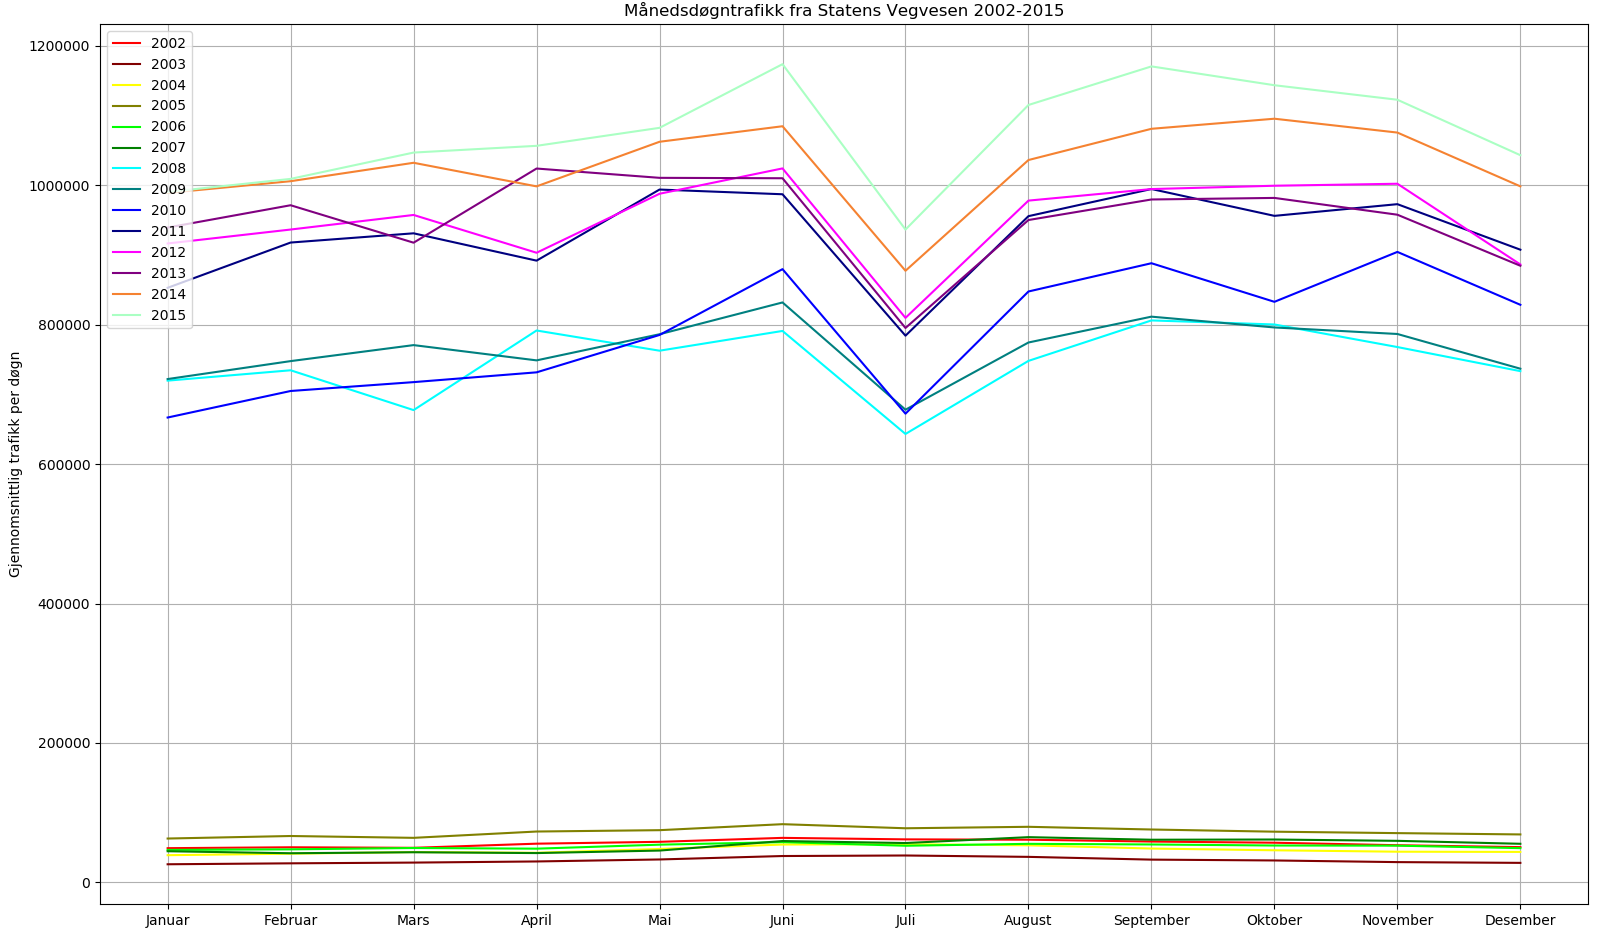
\includegraphics[width=12cm]{xml_02_15_annual_bergen}
%\centering
%\caption{Bergen traffic 2002-2015}
%\label{fig:anualbergen}
%\end{figure}

%\begin{figure}[ht]
%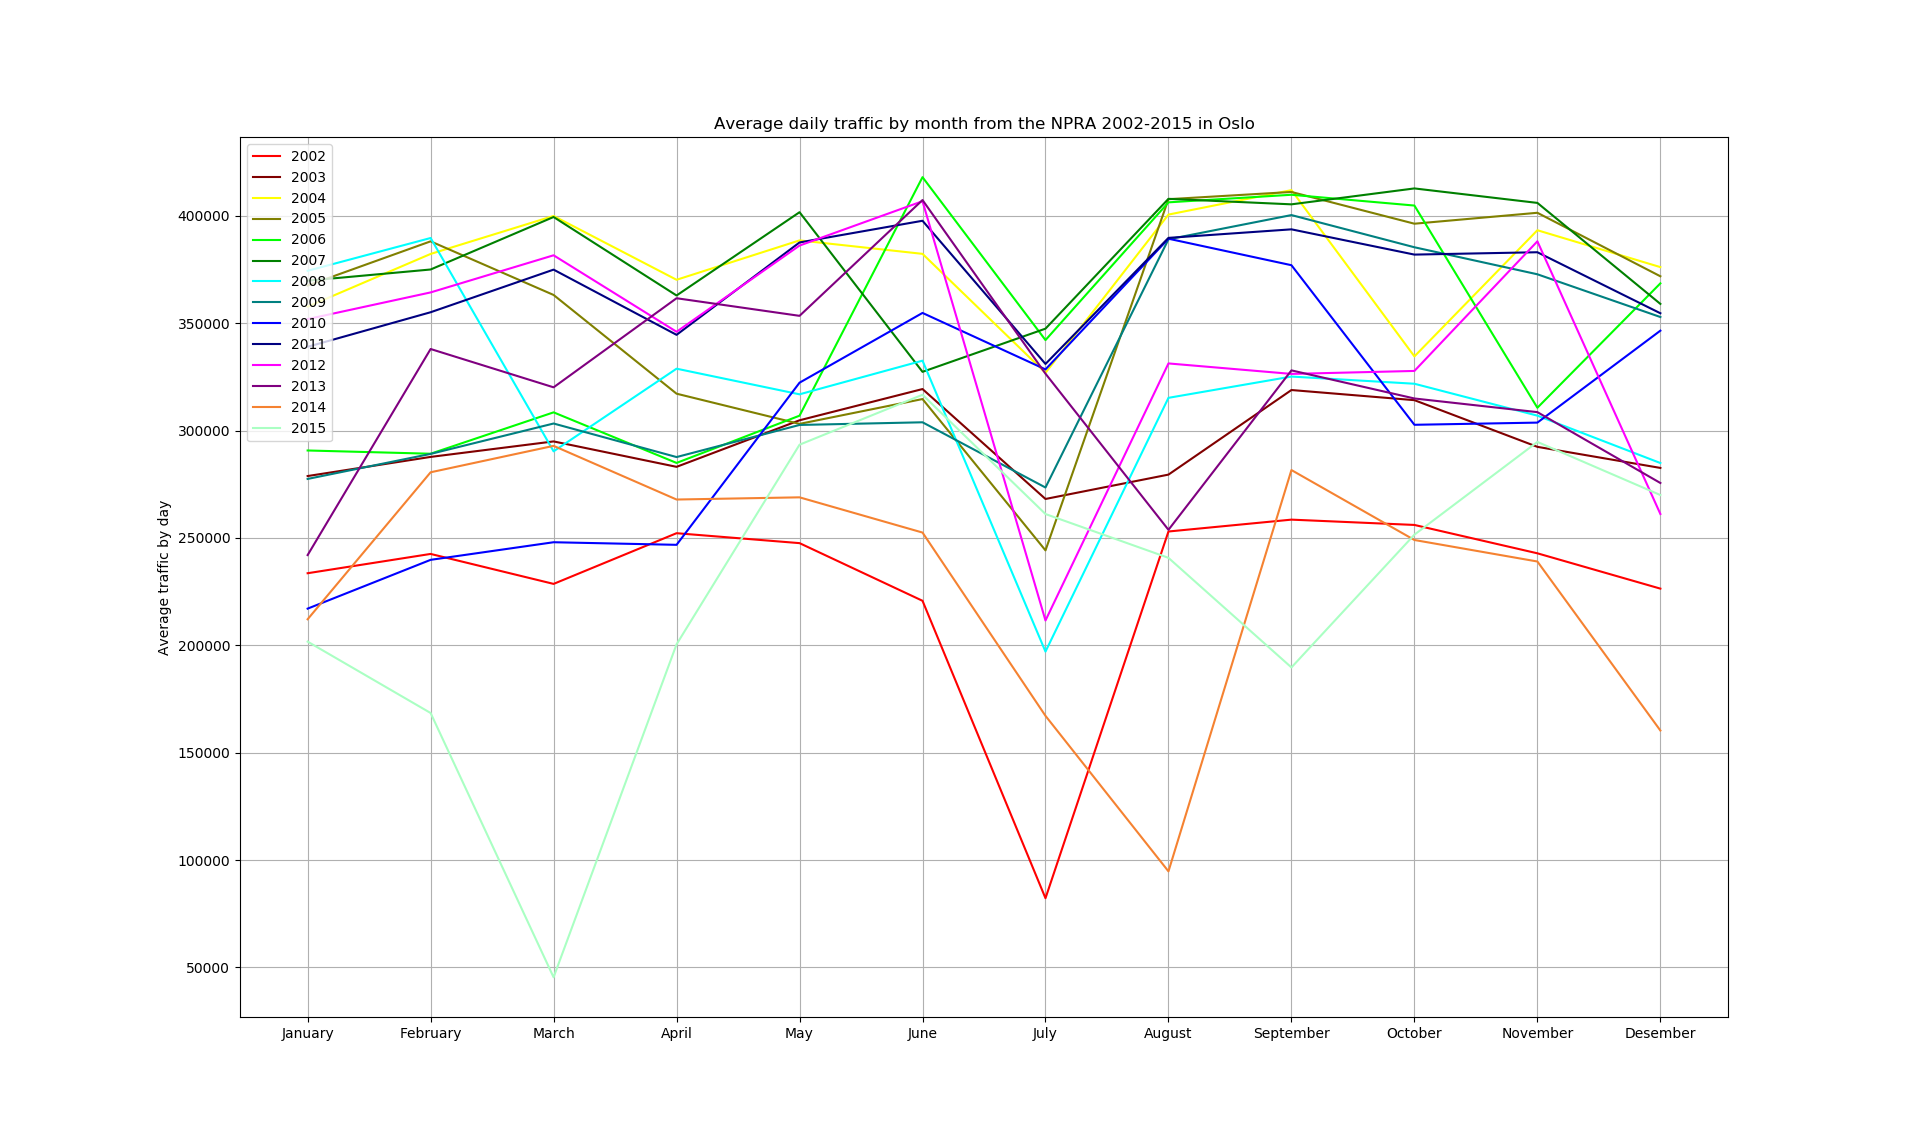
\includegraphics[width=12cm]{xml_02_15_annual_oslo}
%\centering
%\caption{Oslo traffic 2002-2015}
%\label{fig:anualoslo}
%\end{figure}
The dataset is in an XML file structure, a module named NPRA\_monthly.py was created that reads through all rows and collects the relevant columns into an array using Python's openpyxl module and then draws a graph using Python's matplotlib module. For the annual graph, every month of every year was collected. For the towns of Bergen and Oslo the correct roads were identified and then every year of every month of those roads was collected, loaded into an array and then drawn as a graph. The separate text files 'Bergen places.txt' and 'Oslo places.txt' is to make it easy to edit should these roads change in the future. This module when run individually accepts one command argument from the user, either cities of Oslo or Bergen may be provided to specify interest, if no argument is given the annual graph will show. The problem of using these datasets is that the data is an average calculation of monthly traffic, meaning the temporal bounds are too coarse for comparison against the influenza data which in turn is on a weekly basis. For these reasons no figures of this dataset are shown in this thesis (except figure \ref{fig:anualtotal}), they are however available as modules in the directory backend/NPRA/NPRA\_monthly.py and can be seen in the frontend's main program frontend/gui.py appropriate viewport accessible from the NPRA button.

For the weekly datasets a set of traffic registration stations was needed to define the temporal bounds of each area of interest. Defined are the towns of Oslo, Stavanger, and Bergen, as well as the whole of Norway on a level 1 basis. The level 1 registrations are continuous throughout the year on an hourly basis and is exactly what this thesis requires. The module NPRA\_weekly.py captures these functions and also provides the user with command arguments if run individually. The commands are the cities of Bergen, Stavanger or Oslo, if no commands are given the annual graph of the whole of Norway will be drawn instead.

Figures \ref{fig:weeklybergen}, \ref{fig:weeklyoslo} and \ref{fig:weeklystavanger} shows the traffic on a weekly basis. This provides a better resolution for better analysis.


\begin{figure}[!htb]
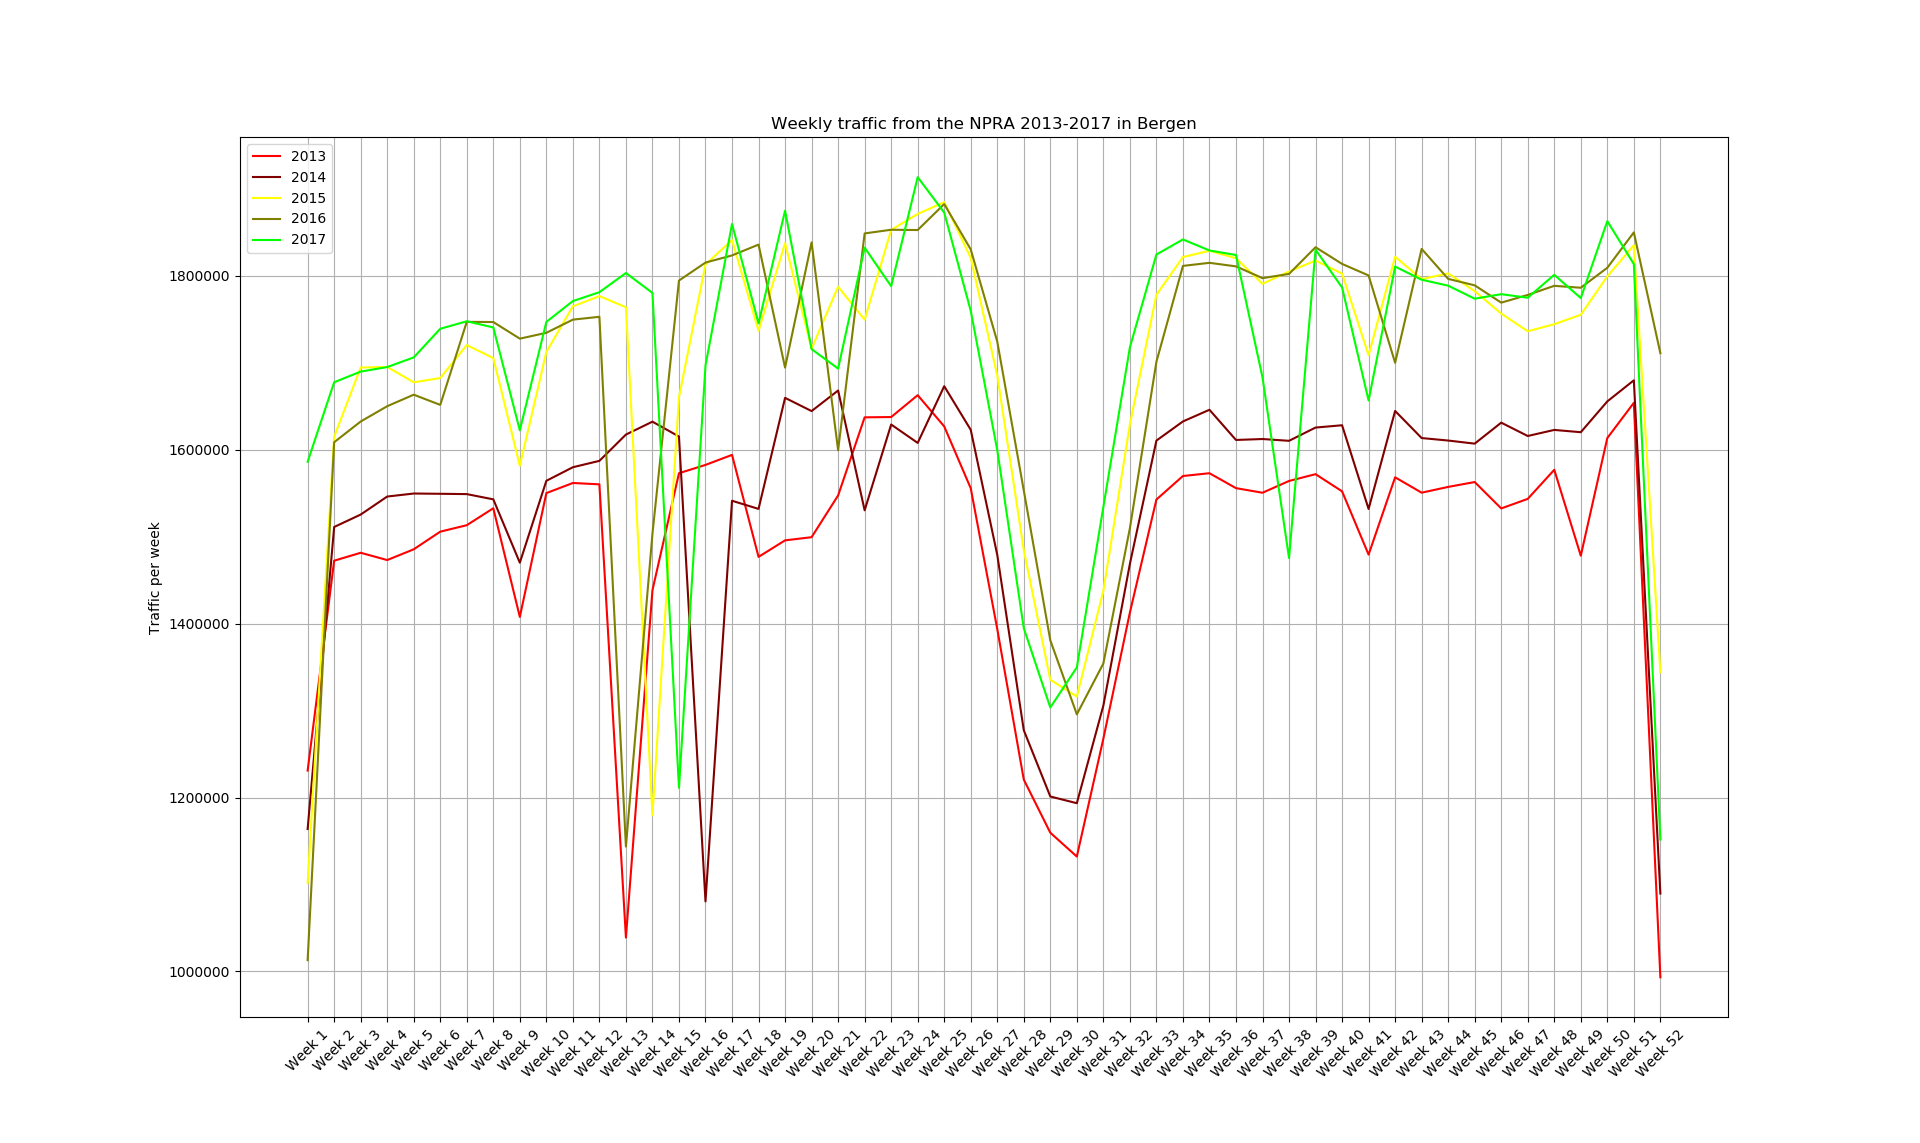
\includegraphics[width=11cm]{NPRA_13_17_weekly_bergen}
\centering
\caption{Weekly data of the city of Bergen}
\label{fig:weeklybergen}
\end{figure}

\begin{figure}[!htb]
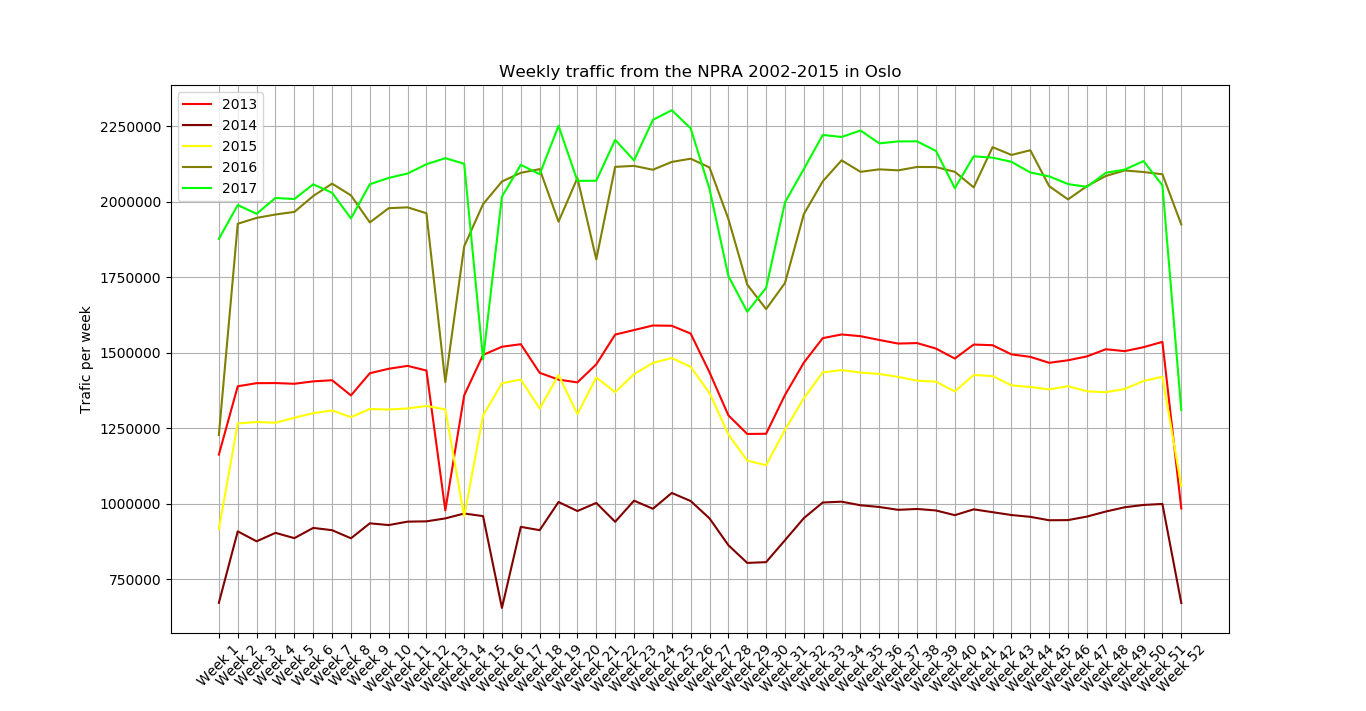
\includegraphics[width=11cm]{NPRA_13_17_weekly_oslo}
\centering
\caption{Weekly data of the city of Oslo}
\label{fig:weeklyoslo}
\end{figure}

\begin{figure}[!htb]
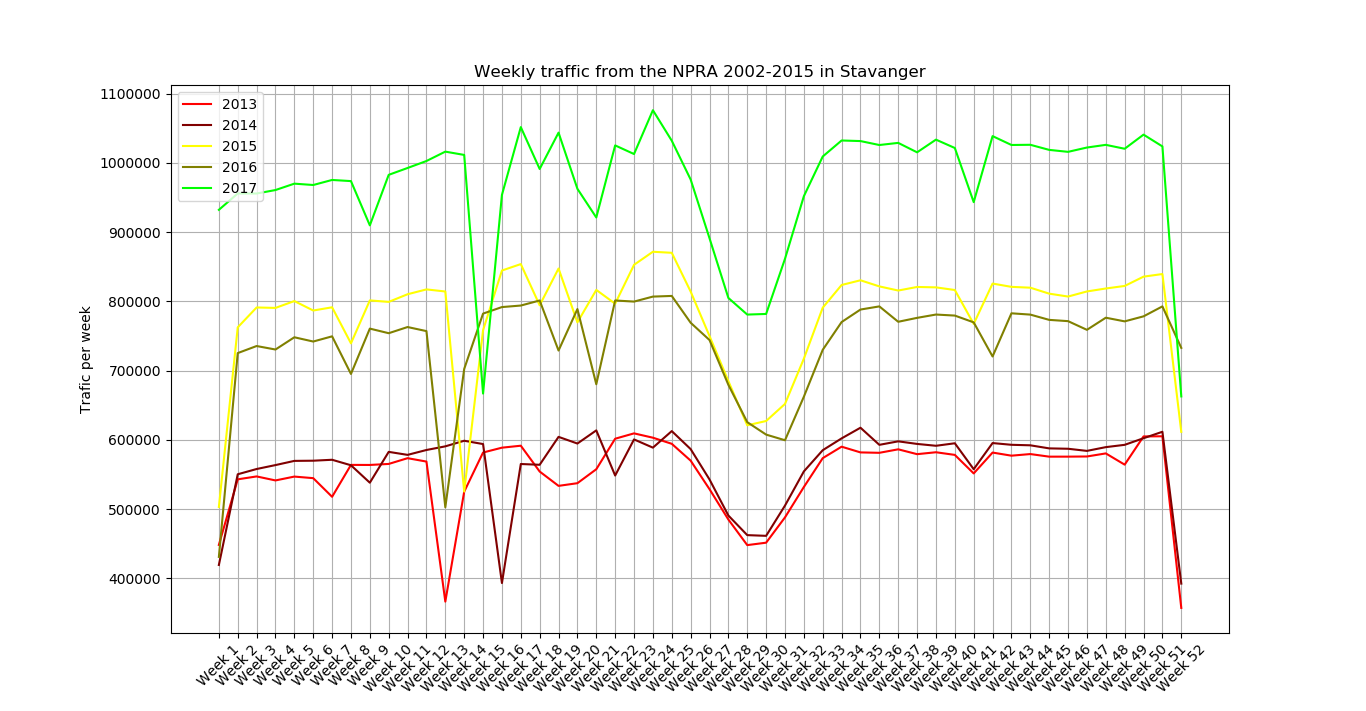
\includegraphics[width=11cm]{NPRA_13_17_weekly_stavanger}
\centering
\caption{Weekly data of the city of Stavanger}
\label{fig:weeklystavanger}
\end{figure}

\newpage

The last NPRA dataset acquired was raw hourly data from a defined subset of all of NPRA's traffic registration stations previously used, this is because the NPRA would only provide this much data from their stores. The data contains all whole hours from all weeks over several years, number of fields available on the road (vehicle lanes, usually only two for regular roads), and how many vehicles passed by that hour and also their lengths in category. Figure \ref{fig:hboundsbergen}, \ref{fig:hboundsoslo} and \ref{fig:hboundsstavanger} shows the different geospatial hourly based bounds (traffic registration stations) used. There are two modules dedicated to the hourly datasets, the NPRA\_Traffic\_Stations\_Graph.py and the NPRA\_Traffic\_Stations\_load\_data.py found in the directory \\
Backend/NPRA/Traffic\_registration\_stations/hourly\_datasets. The graph module is responsible for drawing a graph with specifications of hour to/from, weekday to/from, month to/from, year and field. The load data module is responsible for providing the graph with all the functions it needs to operate, like querying the dataset, the variance of the queried dataset, extracting the dataset from file and organizing it into a data structure, and reading and handling the coordinates of the traffic registration stations so that it can be shown on the map. These last hourly based datasets provide high quality information and is presented in the GUI, by clicking the NPRA button, where the user can try different queries to find different information, more explanations follow in the frontend section of this chapter.

\newpage

\begin{figure}[!htb]
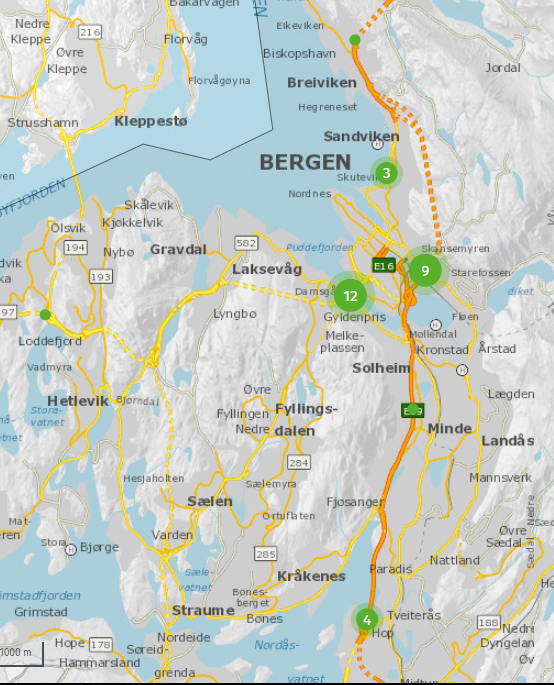
\includegraphics[width=8cm]{times_nivaa1_BERGEN}
\centering
\caption{Geospatial hourly bounds of Bergen, used for hourly data. The green dots show the location of traffic registration stations chosen}
\label{fig:hboundsbergen}
\end{figure}

\begin{figure}[!htb]
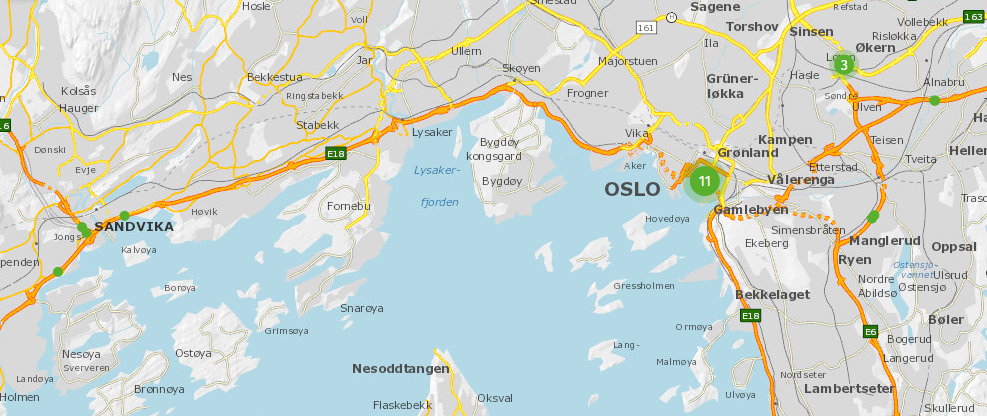
\includegraphics[width=8cm]{times_nivaa1_OSLO}
\centering
\caption{Geospatial hourly bounds of Oslo, used for hourly data.}
\label{fig:hboundsoslo}
\end{figure}

\begin{figure}[!htb]
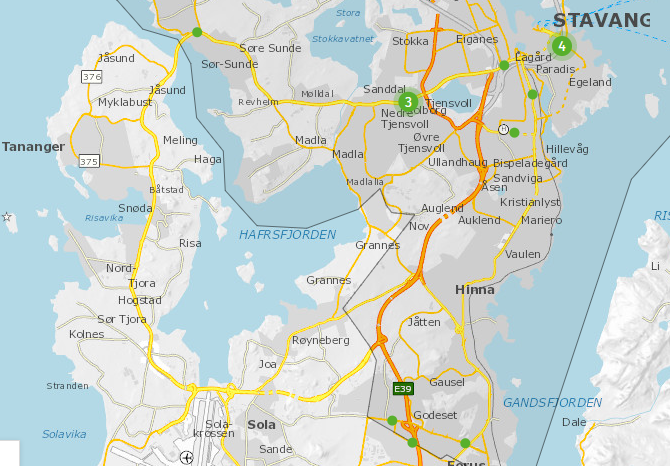
\includegraphics[width=8cm]{times_nivaa1_STAVANGER}
\centering
\caption{Geospatial hourly bounds of Stavanger, used for hourly data.}
\label{fig:hboundsstavanger}
\end{figure}


\newpage



\subsection{Twitter}
Using the representational state transfer (REST) application programming interface (API) it was paramount that in order to build a sufficient dataset, acquiring and collecting data had to begin as soon as possible in order to collect enough data for this thesis. A simple python module was created that takes the input of the API keys provided by the file keys.txt and the keywords to be searched upon provided by the file search\_terms.txt. Explanation on how to create the API key is found in the file backend/twitter/README.md. The program ensures that some duplicate messages are ignored but not all (explained more in the following chapter), and the limit of a hundred tweets dictated by the REST API user agreement was overcome simply by searching for yet another hundred from the last date of the previous hundred until the date limit of about 10 days was reached.\\
The output is appended to a file in this data structure on new lines: id, date, location, tweet, there is also a dotted separator for each new tweet making it more easy for humans to read. The functions described are implemented by the file twitter\_searching.py, which can be run as its own module and saves new tweets to the file twitter\_data.txt.

A straightforward analysis tool for the Twitter data in the file twitter\_data.txt was created by simply counting how many tweets there are. The idea is that during influenza seasons numbers of influenza-related tweets increases and then decrease when off the season, while the number of non-relevant tweets is constant during the whole year (or slightly increasing or decreasing based on the popularity of Twitter as a social media). A more complex tool for analysing the tweets for relevance was elected to bee too much work for this thesis. The advantage of simply counting how many possible tweets there are is that it is fast and easy to implement, the drawback is that it captures non-relevant tweets. Future work may be done to improve this quality with a better analysis tool. 

\begin{figure}[ht]
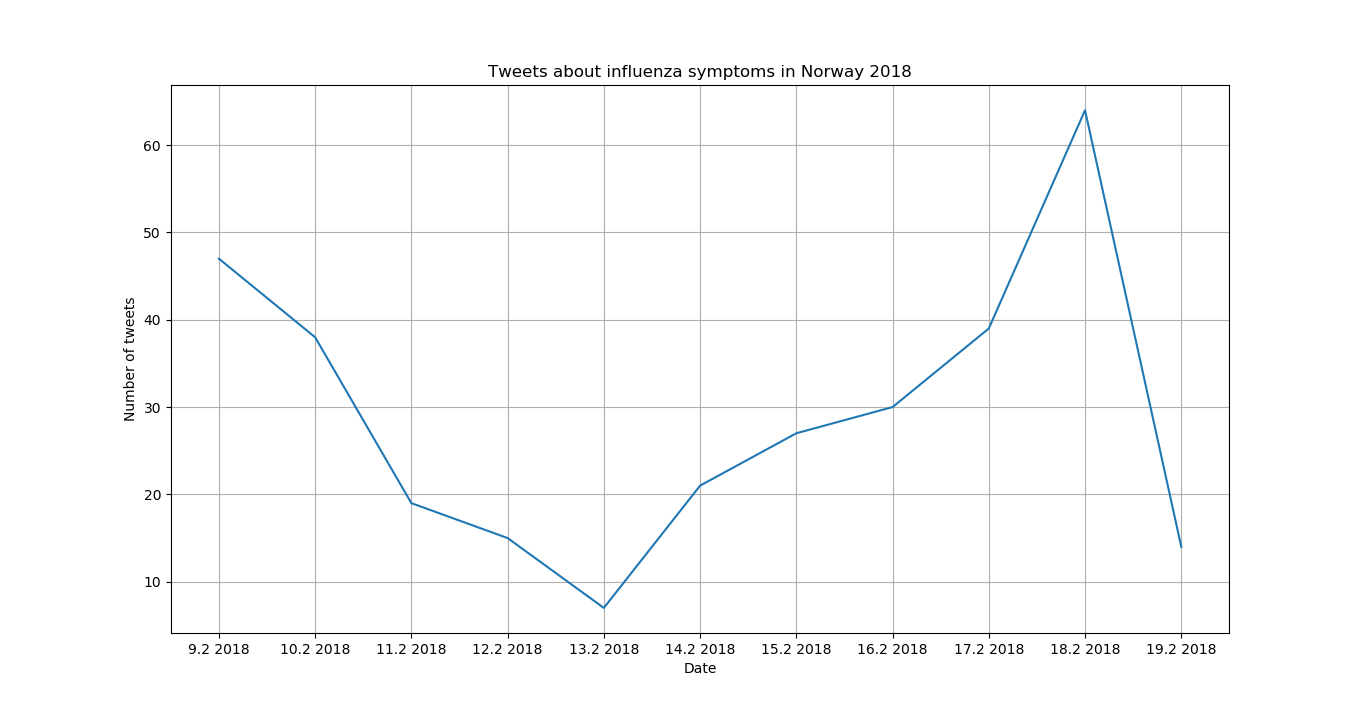
\includegraphics[width=16cm]{twitter_tweets_2018}
\centering
\caption{Tweets concerning ILS of 2018}
\label{fig:twitterAnal}
\end{figure}

Figure \ref{fig:twitterAnal} shows the results of the time-frame captured. The analysing function is implemented in the file twitter\_analyser.py, when the module is executed on its own it shows a graph over the data found in the file twitter\_data.txt.\\
A simple batch file twitter.bat was created to make it easy running these programs in the desired order. This module requires manual updates by running the individual module itself in the directory backend/twitter/twitter.bat. If no API key is provided the Twitter graph can still be viewed in the frontend main program frontend/gui.py's appropriate viewport accessible from the Twitter button, but it cannot append new updates without this key.


\newpage





\subsection{Kolumbus}
The data provided by Kolumbus was in a .png format needed to be converted into a more convenient (and appropriate) data structure. The chosen data structure conversion was comma separated values (CSV) stored in the delimited text file '15\_17\_månedstall\_total.csv'. From there it was a simple job to plot the data in a python script, unfortunately the data is only on a monthly basis which is too coarse a temporal aggregation to derive anything useful for this thesis. Figure \ref{fig:kolumbus_15_17} shows the results.

\begin{figure}[!htb]
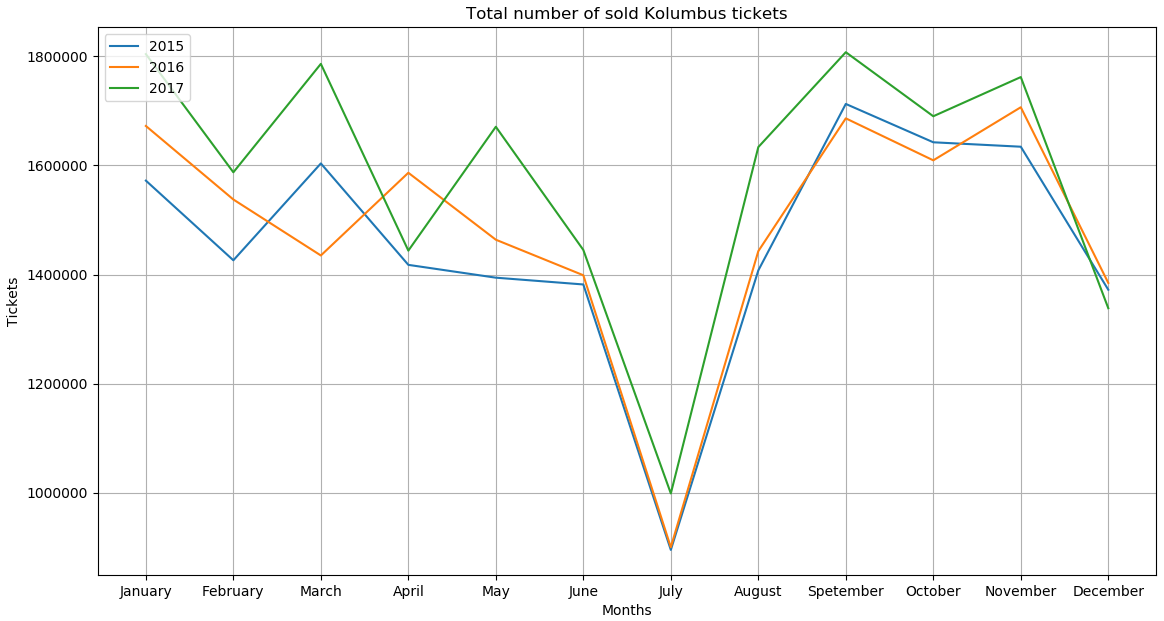
\includegraphics[width=8cm]{kolumbus_total_num_sold_15_17}
\centering
\caption{Monthly passenger travel with Kolumbus}
\label{fig:kolumbus_15_17}
\end{figure}




\subsection{Ruter}
The data provided by Ruter was in a .xlsx file and could easily be read, extracted and plotted by a simple python script. Figure \ref{fig:ruter_15_18} shows the results. Consider that with Python's matplotlib module, mounted in the frontend's main program frontend/gui.py, a user can zoom in and out to get a more desired and uncluttered view. The data was provided by a daily basis for the years of 2015-2018. Observe that the first year (in blue) is lower because it does not contain Oslo's underground train service passenger data.

\begin{figure}[!htb]
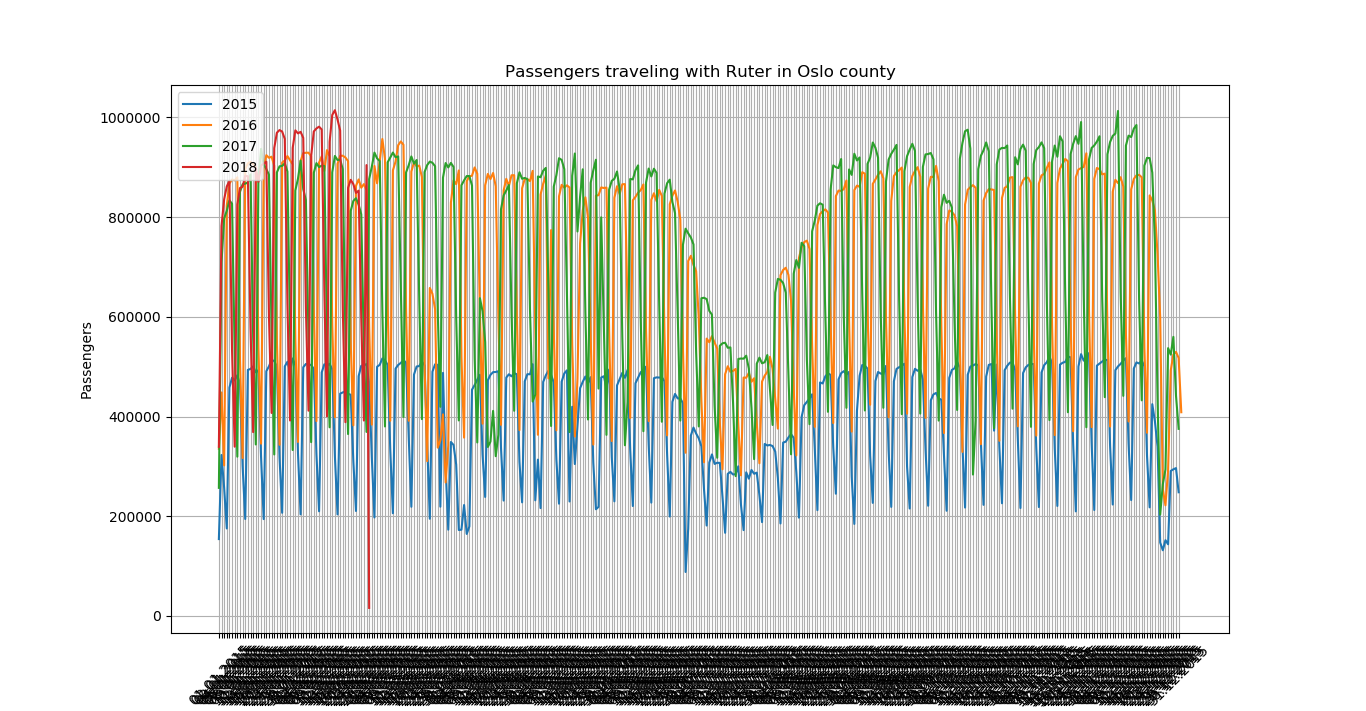
\includegraphics[width=13.5cm]{ruter_15_18}
\centering
\caption{Daily tickets sold with Ruter, the year of 2015 does not contain Oslo's underground train service passenger data}
\label{fig:ruter_15_18}
\end{figure}

\newpage










\section{The Frontend}
The thesis's program is divided into two: The backend and the frontend. The frontend is responsible for visualising the data provided by the backend. It does so by mounting a graphical user interface (GUI) that provides everything the user needs from this thesis. The GUI uses other frontend modules described in the following subchapters. Figure \ref{fig:frontend_diagram} shows a diagram of the frontend.

\begin{figure}[h]
\includegraphics[width=15cm]{frontend_diagram}
\centering
\caption{A semi detailed diagram of the Frontend structure and functions}
\label{fig:frontend_diagram}
\end{figure}

\subsection{The GUI}
The file gui.py is the main program. It mounts the GUI with help from backend modules and the frontend modules such as the file map\_canvas.py, the file scrframe.py, the file double\_y\_graphs.py, the file NIPH\_frame.py and the file NPRA\_frame.py . The GUI is created using Python's standard Tkinter module (standard meaning it's not a required external library), and it provides the means of a basic window creation with all the other usual GUI necessities available. 

The program gui.py is structured in two parts: The buttons frame and the data frame. The buttons frame produces a menu and simply makes available buttons to be clicked upon showing the different graphs for the respective datasets from the backend. The data frames show the graphs and if needed a map, visualizing the data from the backend. The backend takes time to load, to make this experience more user-friendly a progress bar is shown progressing relative to the actual loading sequence. Upon completion, the NIPH data is shown as a default view. The user may use the mouse wheel to scroll up and down the view and click the buttons to change datasets. 

In some datasets, a map is provided for further visualisation. the map is interactive with its own buttons and also responds to dragging the mouse in order to move the map, double-clicking in order to zoom in and using the mouse wheel, when hovering over the map, to zoom in and out. Figure \ref{fig:the_gui} shows the GUI.

\begin{figure}[!htb]
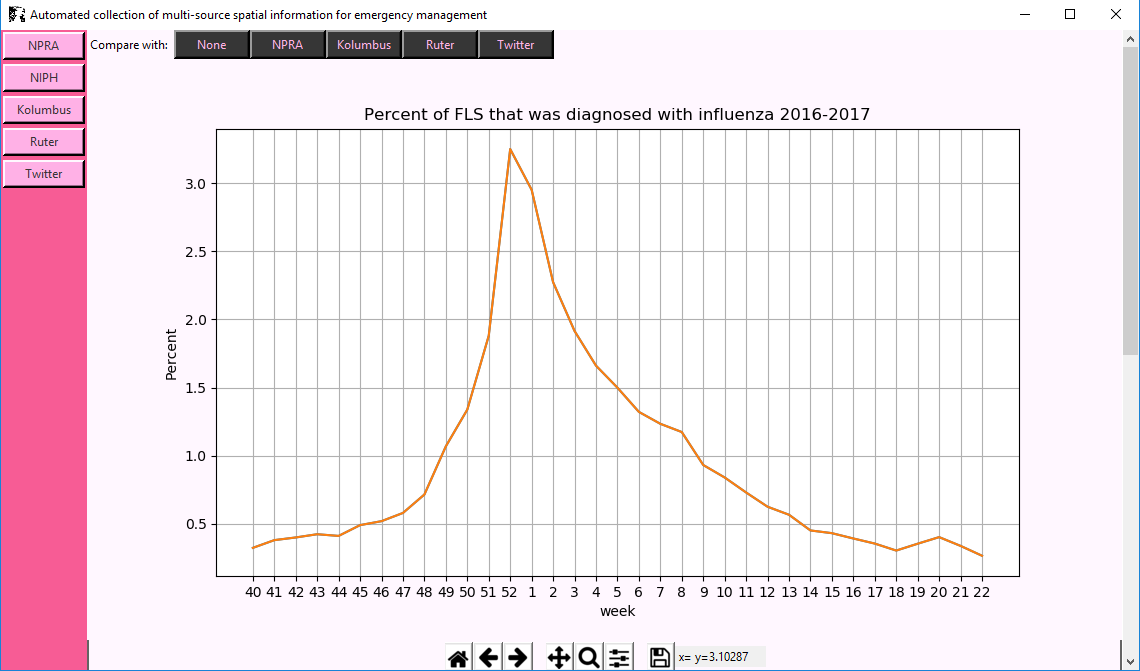
\includegraphics[width=12cm]{the_gui}
\centering
\caption{The GUI}
\label{fig:the_gui}
\end{figure}



\subsection{The Map}
The file map\_canvas.py provides the GUI a Goompy\cite{goompy} map on a Tkinter canvas. This file is also from the Goompy project, but is heavily modified to serve the purpose of this thesis. The file launches a Google static API map on a Tkinter canvas and provides basic Google map functions and user input. The functions edited for this thesis is: better zooming capabilities, coordination markers with individual colors and sizes, ability to focus on the map by will and some other minor bug fixes.

\subsubsection{Goompy}
Goompy\cite{goompy} is an open Github project and provides an interactive Google static map\cite{googleSM} for Python, it was created by Simon D. Levy. The main program uses this map implementation with it's own significant modifications to serve an interactive Google based map solution in order to provide visualisation of information.\\
The core Goompy file is found in the directory of /Frontend/goompy/\_\_init\_\_.py. This was heavily edited to provide the necessary functions of this thesis. The edit includes: Multithreading the fetching of Google static map images thus making Goompy about four times faster, dragging now changes latitude and longitude based on x and y position of the map to better help zooming functions, having the API key fetched from a separate text file in order to hide this from misuse by other developers, support of optional map coordinates to be plotted directly in the Google static map API, using and drawing a list of coordinates as a diamond-shaped polygon with individual colors and sizes and using the mouse wheel to zoom in and out.\\
The initial build fetched about one image per second in order to not exceed Google's throttle request quota. Upon further investigation this quota is set to ten QPS (queries per second) which means such a high buffer can be exploited. By converting the image extraction algorithm to be multi-threaded, fetching map fragments was increased to 4 - 6 images per second, well below Google's QPS and significantly strengthening the user experience by having a more responsive program.\\
Goompy requires a Google static map API key in order to work properly, users are asked to create the file Frontend/api\_keys.txt and paste the key there as described by the file Frontend/README.md. The original project saved the Google map images in a cache so that fetching a specific map with a familiar geolocations would be instantaneous instead of fetching them again from the Google server, this however was a violation of the terms of agreement and that function was removed from this thesis. Caching resources is a good way to quickly get often used functions, although the new implementation changes latitude and longitude often, as it allows this change, this is no longer a good strategy. For these two reasons the caching was removed.
Figure \ref{fig:the_goompy} shows the Goompy map interface. In the top left corner radiobuttons change the current viewing map type. The buttons to zoom in and out are found in the bottom right corner.

\begin{figure}[!htb]
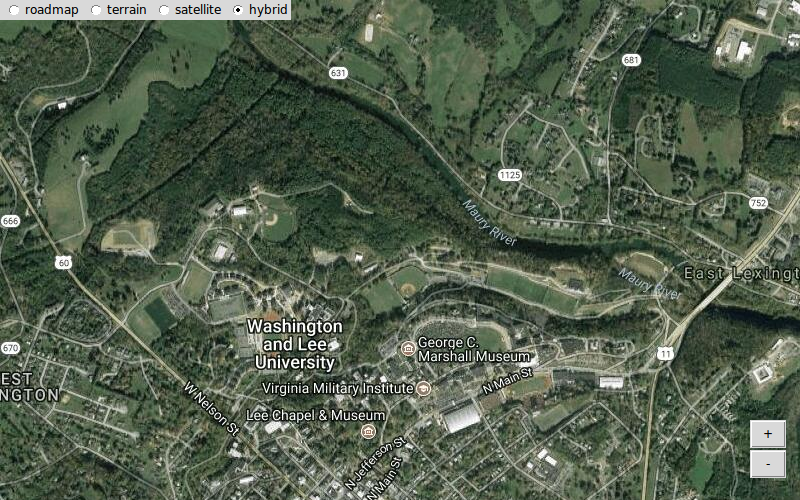
\includegraphics[width=12cm]{goompy}
\centering
\caption{A Goompy implementation of Google's static map API}
\label{fig:the_goompy}
\end{figure}

\newpage














\subsection{The Scrollbar}
Creating a functional scrollbar that responds to mouse dragging and mouse wheel events in Tkinter proved difficult, which is why Eugene Bakin's Tkinter scollable\cite{scrframe} frame was used. It is an open Github project. The file Frontend/scrframe.py contains his code with minor edits in order to be able to scroll with the mouse wheel, get the Tkinter focus, resetting scrollbar viewport and better resizing of the window. This module may also be run independently for testing purposes.




\subsection{NIPH dataframe}
The GUI module is structured in two parts: The buttons frame and the data frame, data frames visualise information from the backend. The NIPH data frame was created as it's own module to better organise code, the module serves as an easily implemented dataframe for the main program gui.py. The NIPH data frame was extended with the functionalities that allows for comparison of the NIPH data with all the other datasets at the different influenza seasons available. The frontend module NIPH\_frame.py was created to be implemented by the main file GUI.py and the file double\_y\_graphs.py provides the necessary supportive algorithms. Both files may be run individually for testing purposes. The comparison functions work in the way that the user selects a dataset to compare with by clicking a button in the top border. A drop-down menu will be produced giving the choices of cities and influenza seasons. Two graphs will then be drawn sharing the same x-axis but having different y-axes. This makes for easy comparison and querying the data in order to find possible correlations. While the graphs are loading a label displaying "Loading, please wait ..." will be shown in orange at the very right of the buttons panel. Figure \ref{fig:NIPH_compare} shows the NIPH comparing buttons panel.

\begin{figure}[ht]
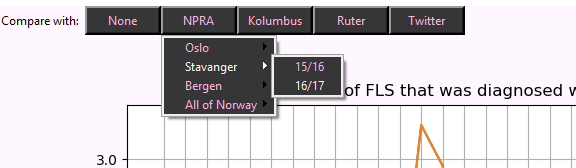
\includegraphics[width=15cm]{NIPH_compare}
\centering
\caption{NIPH comparing buttons panel}
\label{fig:NIPH_compare}
\end{figure}

\newpage

\subsection{NPRA dataframe}
In addition to the monthly and weekly datasets the hourly are presented in its own GUI module implemented by the main file GUI.py. The hourly datasets contains 58 different traffic registration stations from the cities of Bergen, Stavanger and Oslo and may be queried with the buttons-panel. The dropdown buttons provide the choices of hours to/from, weekdays to/from and months to/from from the years of 2013 to 2017 which can be selected from the checkbuttons, then there is a show button which initiates the query, lastly there is a save button which withdraws the data queried and saves it to a .csv file in a chosen directory.\\ The query may take up to a minute loading depending on how many years were selected, a label displaying "Loading, please wait ..." will be shown in orange to the very right of the query panel while the algorithms is running. If the query is invalid a label displaying "Error, invalid request!" will be shown in red at the same position. \\
On the left border a map is shown, displaying the available traffic registration stations in random colors and sizes (more about this in chapter 6). Figure \ref{fig:NPRA_query} shows the NPRA query buttons panel.

\begin{figure}[ht]
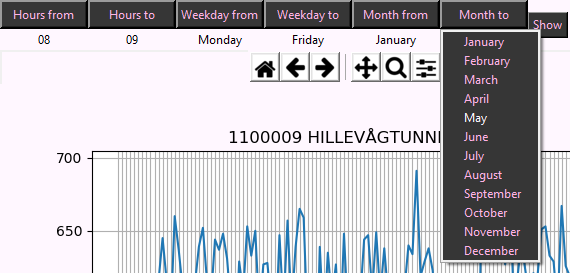
\includegraphics[width=15cm]{NPRA_query}
\centering
\caption{NPRA query buttons panel}
\label{fig:NPRA_query}
\end{figure}




